\chapter{Wstęp}
\section{Wprowadzenie}
Rola automatyzacji w obsłudze klienta znacznie wzrosła w ostatnich latach. Można to zaobserwować w dynamice, z jaką ewoluują systemy informatyczne nazywane elektronicznymi biurami obsługi klienta (eBOK). Takie systemy są szeroko stosowane w różnych branżach sektora usług, takich jak energetyka, wodociągi, telekomunikacja, usługi multimedialne i zarządzanie wspólnotami mieszkaniowymi.

Z punktu widzenia użytkowników główną zaletą eBOKów jest możliwość skorzystania z oferowanych przez nie funkcji w dowolnym miejscu i czasie. Cecha ta nie tylko poprawia jakość obsługi klienta, ale także zwiększa efektywność organizacji wdrażających takie rozwiązanie. Poza zapewnieniem dostępu do informacji o rozliczeniach i płatnościach, eBOKi wspierają także realizację bardziej zaawansowanych procesów, jak zgłaszanie problemów technicznych, zarządzanie zgłoszeniami serwisowymi i komunikację z zarządem. Ważnym aspektem tych systemów jest bezpieczeństwo danych osobowych, które jest zapewniane poprzez regularne aktualizacje systemu, wdrażanie mechanizmów uwierzytelniania dwuskładnikowego oraz zgodność z przepisami o ochronie danych osobowych, takimi jak RODO.

Obecnie na rynku spotkać można wiele systemów typu eBOK. Jednym z nich jest system ,,Energa24''. Umożliwia on klientom dostęp do informacji o zużyciu energii, przeglądanie i pobieranie rachunków, dokonywanie płatności online oraz zgłaszanie awarii~\cite{energa}. Standardowy scenariusz dokonywania płatności za pomocą tej aplikacji pokazano na Rysunku \ref{fig:energa_manual}. Użytkownik może wybrać odpowiedni rachunek, a następnie poprzez bezpieczną bramkę płatności uiścić należności bezpośrednio w systemie.

\begin{figure}[htb]
	\centering
		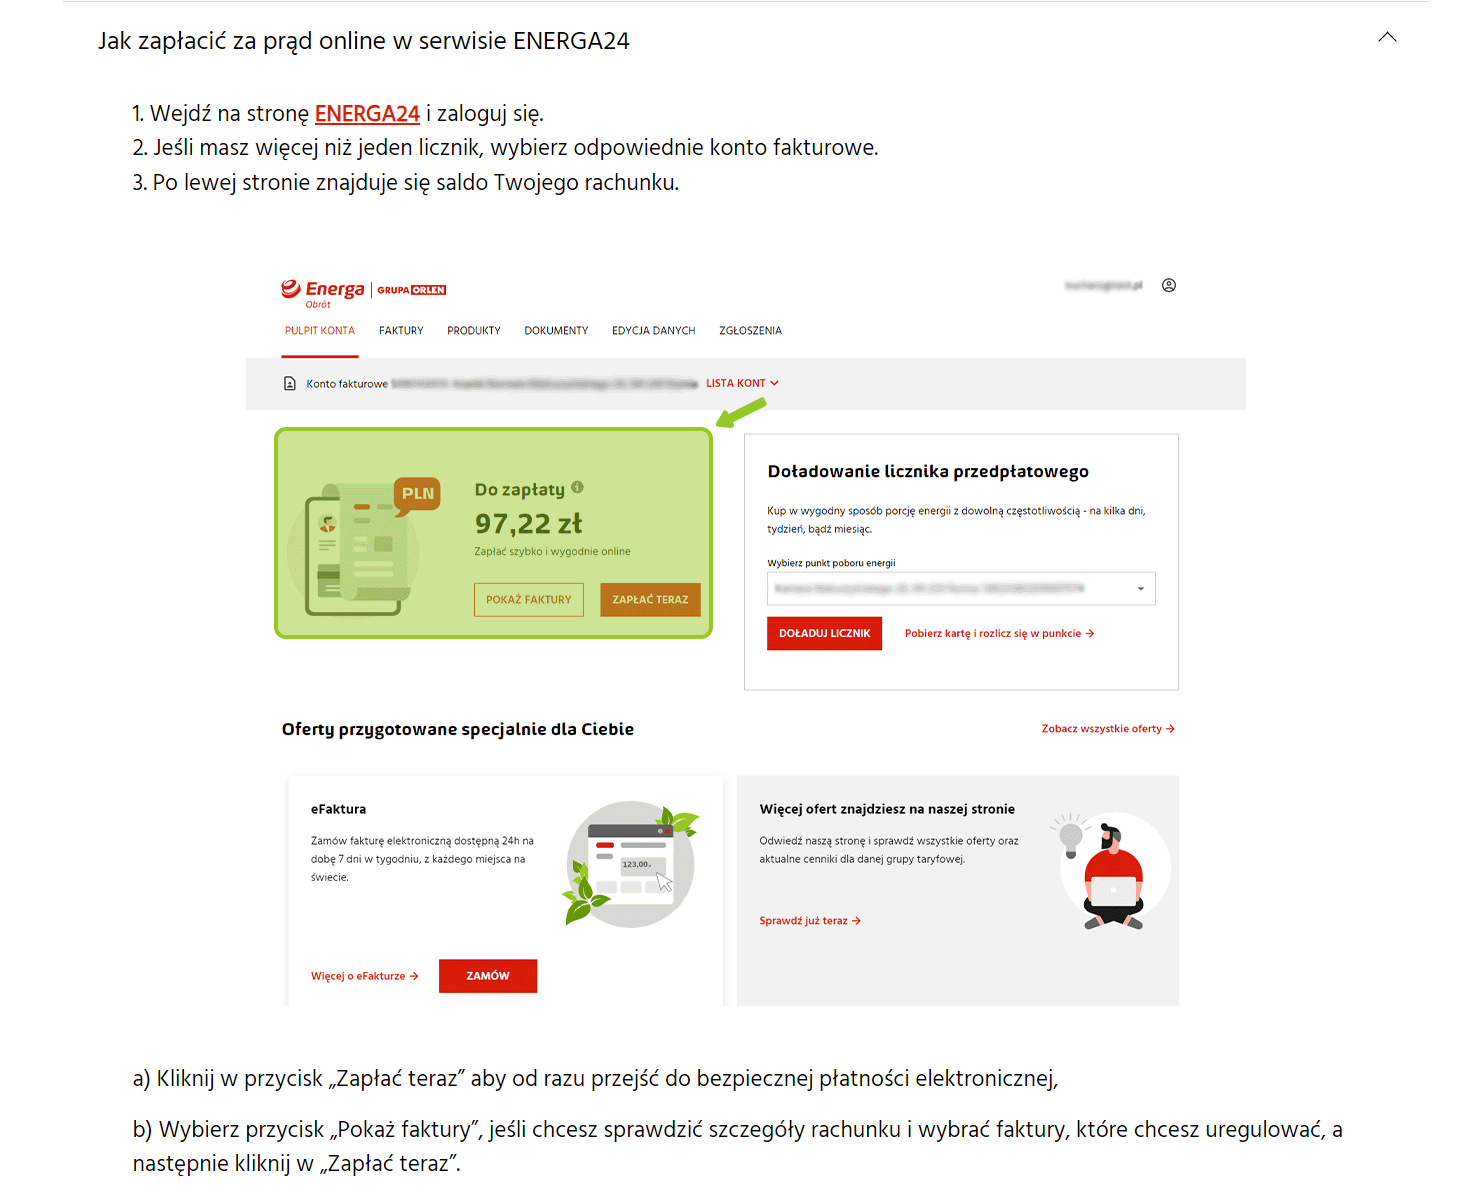
\includegraphics[width=0.85\linewidth]{rys01/energa_manual_1.png} \\[-1ex]
		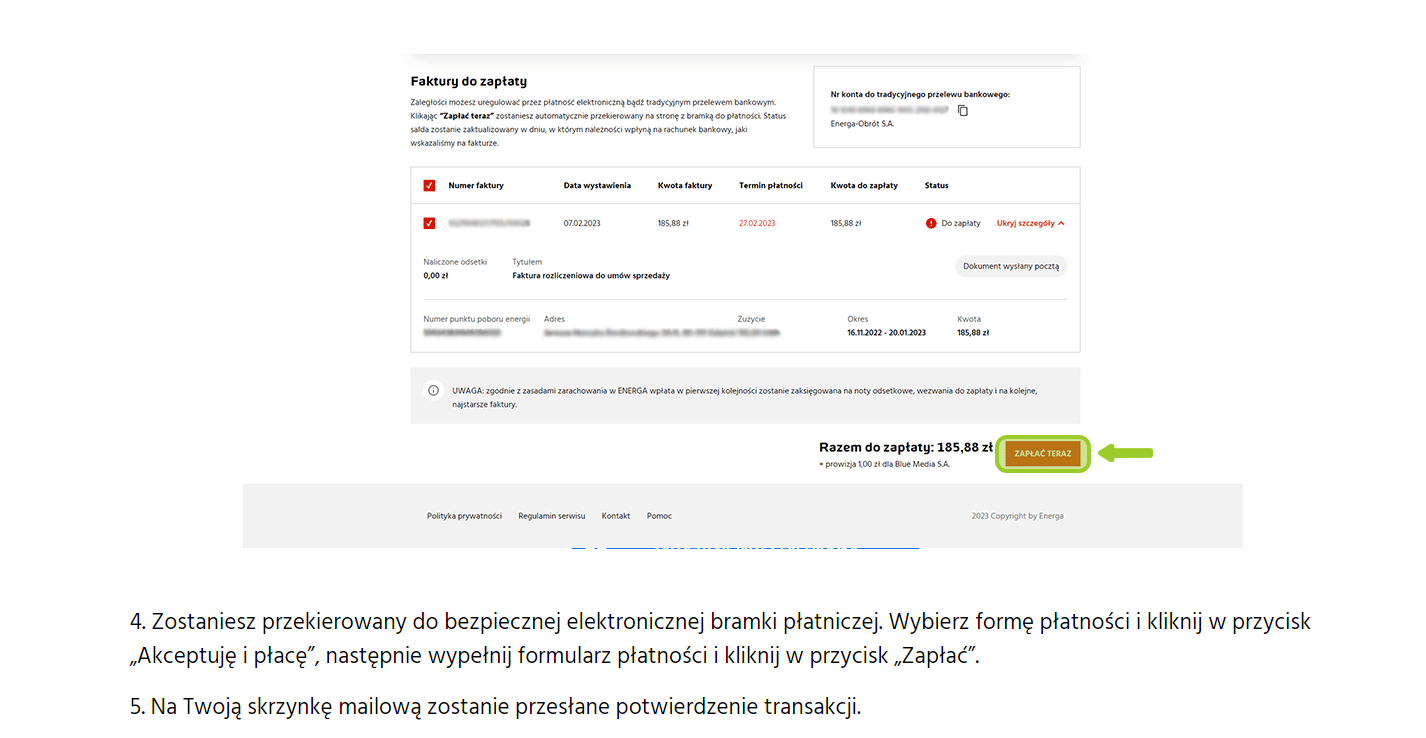
\includegraphics[width=0.85\linewidth]{rys01/energa_manual_2.png} \\[-1ex]
		\caption{Opis scenariusza dokonania płatności za energię elektryczną w serwisie ,,Energa24''~\cite{energa}}
	\label{fig:energa_manual}
\end{figure}

Innym przykładem systemu eBOK jest rozwiązanie dostarczane przez operatora telekomunikacji Play, który umożliwia użytkownikom zarządzanie usługami telekomunikacyjnymi oraz multimediami. System ,,Play24'' oferuje szeroki zakres funkcji, takich jak monitorowanie zużycia internetu, minut rozmów czy SMS-ów, co pozwala użytkownikom na bieżąco śledzić stan swoich pakietów i w razie potrzeby dokupować dodatkowe usługi. Użytkownicy mogą również sprawdzać historię swoich aktywności, w tym szczegółowe informacje na temat wysyłanych wiadomości, połączeń czy zakupionych pakietów ~\cite{Play24}.

System ,,Play24'' pozwala także na łatwe i szybkie regulowanie płatności za usługi telekomunikacyjne, oferując różnorodne metody płatności, w tym Google Pay, Apple Pay oraz BLIK. Użytkownicy mogą skonfigurować automatyczne płatności, co znacząco upraszcza zarządzanie opłatami. Dodatkowo, aplikacja umożliwia dostęp do szczegółowych faktur oraz wyciągów z historii transakcji, co ułatwia kontrolowanie bieżących wydatków.

Co więcej, system ten umożliwia zarządzanie usługami światłowodowymi, w tym zdalne restartowanie routera czy zmianę hasła do Wi-Fi. W przypadku problemów technicznych, użytkownicy mogą zgłaszać usterki i diagnozować problemy bezpośrednio z poziomu aplikacji. Dzięki intuicyjnemu interfejsowi, użytkownicy mogą szybko przemieszczać się między funkcjami aplikacji, co znacząco usprawnia zarządzanie usługami telekomunikacyjnymi i technicznymi.

Rysunek \ref{fig:play24_manual} ilustruje te funkcje, jak użytkownicy mogą śledzić swoje zużycie internetu, zarządzać opłatami oraz kontrolować ustawienia sieci domowej, co zwiększa ich komfort użytkowania oraz zapewnia większą kontrolę nad korzystaniem z usług.

\begin{figure}[ht]
    \centering
    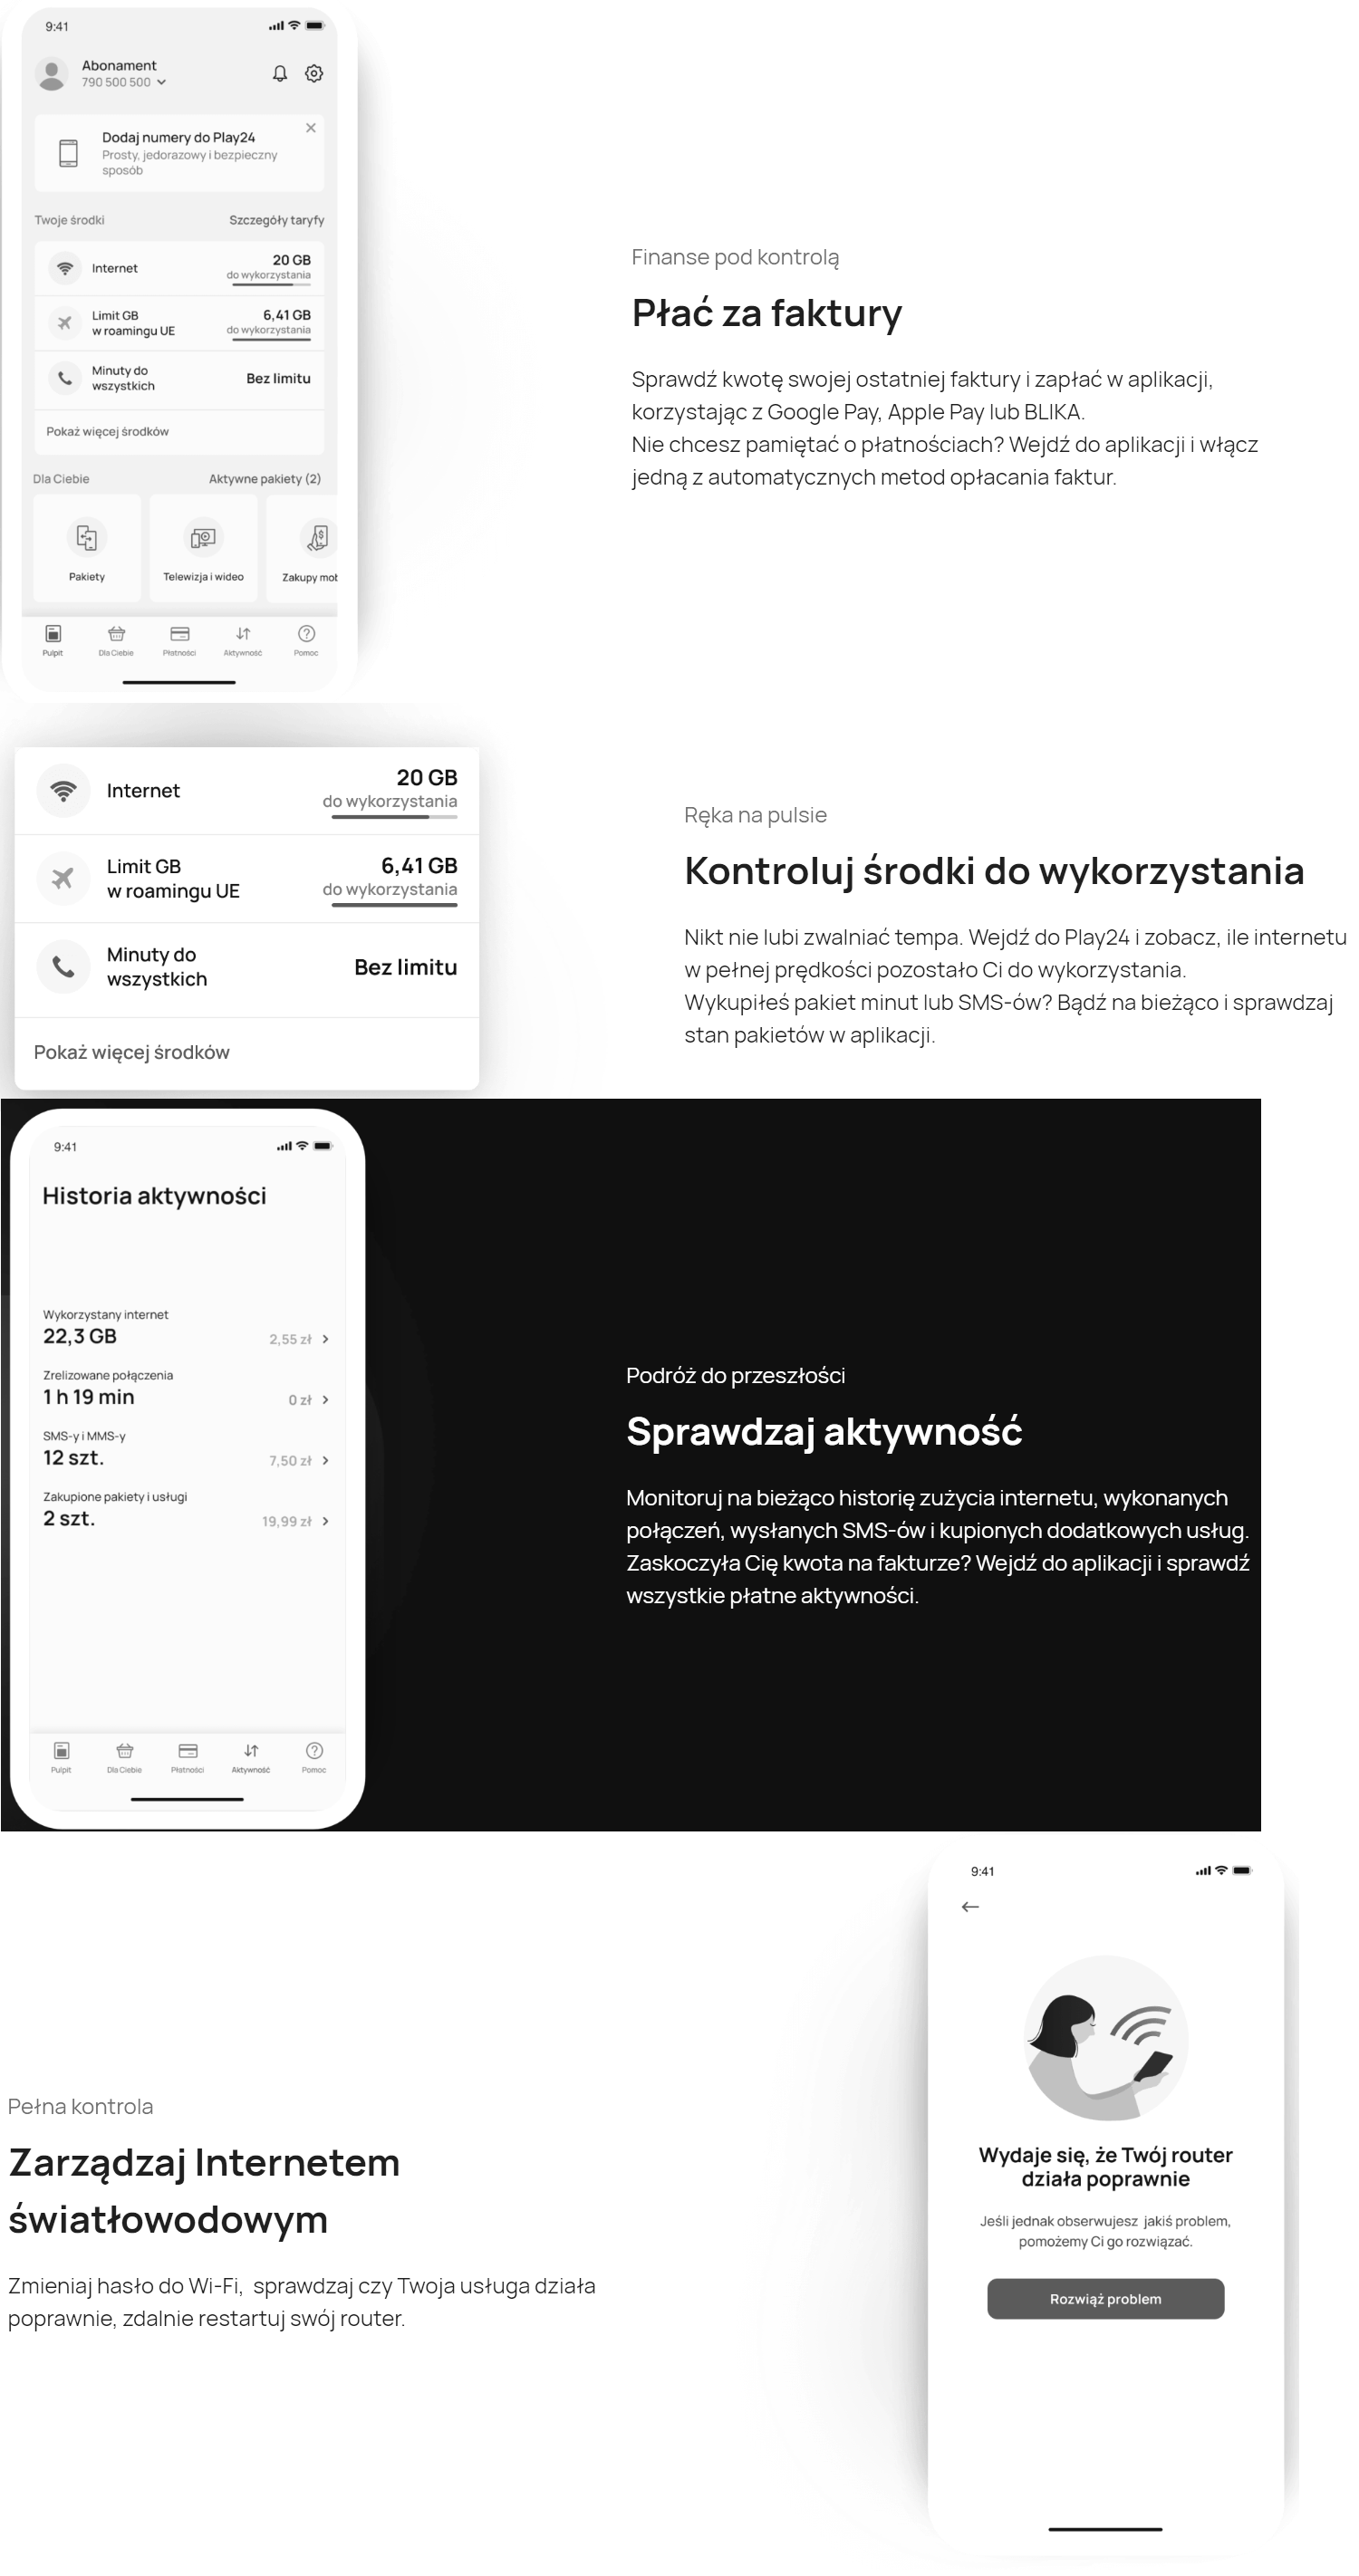
\includegraphics[width=0.6\linewidth]{rys01/play_manual}
    \caption{Opis głównych funkcji oferowanych w systemie ,,Play24''}
    \label{fig:play24_manual}
\end{figure}

Dostępne są również rozwiązania dostosowane specjalnie do potrzeb spółdzielni i wspólnot mieszkaniowych. Przykładem może być system ,,e-Kartoteka'', który umożliwia mieszkańcom zarządzanie zgłoszeniami usterek oraz podgląd postępu zgłoszenia, wgląd oraz regulację w płatności za nieruchomość, wgląd w dokumenty nieruchomości oraz wspólnoty, głosowanie nad uchwałami wspólnoty, a także komunikację z zarządem~\cite{e-kartoteka}. System ten oferuje również możliwość przeglądania rozliczeń mediów, takich jak woda, energia elektryczna czy ogrzewanie, co ułatwia mieszkańcom śledzenie swoich bieżących opłat i zużycia. Aplikacja ,,e-Kartoteka'' umożliwia również mieszkańcom szybki dostęp do wyciągów z rachunków i opłat miesięcznych, w tym szczegółowych rozliczeń za media (patrz rysunek~\ref{fig:kartoteka_manual}). Dzięki intuicyjnemu interfejsowi użytkownicy mogą sprawnie poruszać się między funkcjami, takimi jak tablica ogłoszeń, forum dyskusyjne dla mieszkańców czy dokumentacja nieruchomości, co znacząco poprawia komunikację i współpracę w obrębie wspólnoty. Ponadto mieszkańcy mają możliwość zgłaszania odczytów liczników, co automatycznie generuje informacje na temat aktualnego stanu rozliczeń oraz zaległych opłat, podobnie jak widoczne na przedstawionym obrazie funkcje raportowania stanu liczników i przeglądania historii faktur.
\begin{figure}[ht]
    \centering
    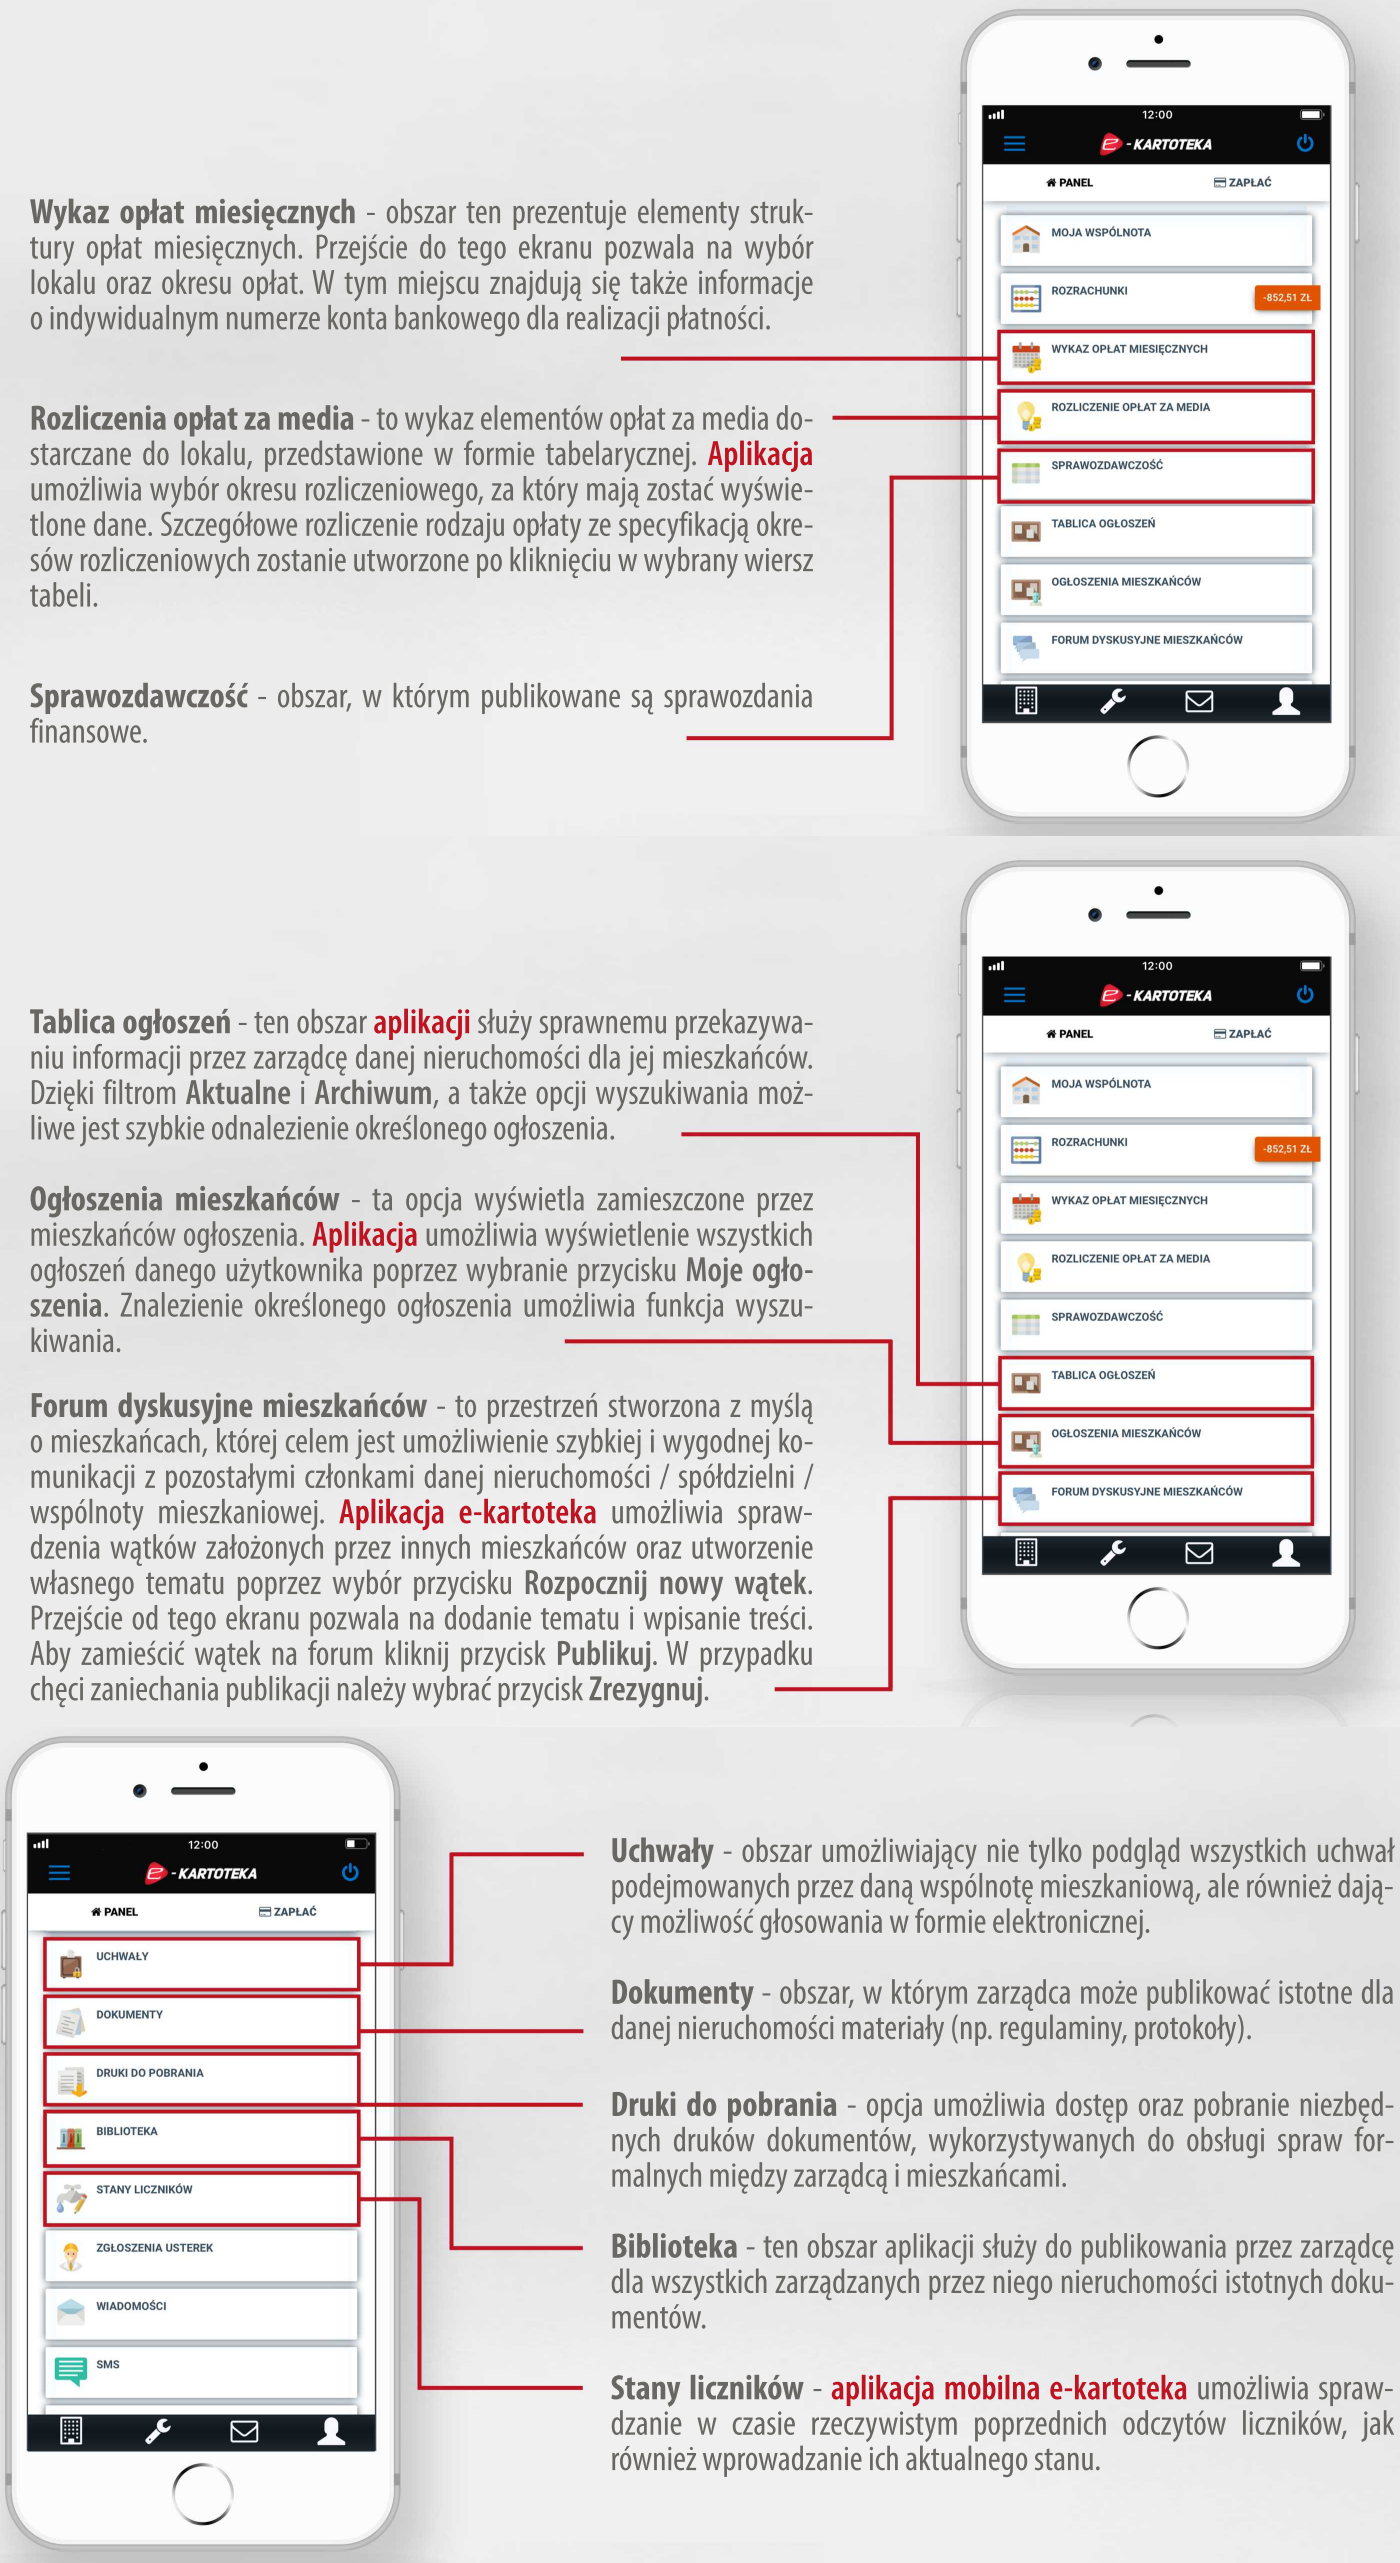
\includegraphics[width=0.6\linewidth]{rys01/kartoteka_manual}
    \caption{Opis głównych funkcji oferowanych w systemie ,,e-Kartoteka''~\cite{e-kartoteka_manual}}
    \label{fig:kartoteka_manual}
\end{figure}

Systemy eBOK różnią się pod względem funkcji, skalowalności oraz stopnia integracji z innymi rozwiązaniami, takimi jak narzędzia płatności online, systemy zarządzania nieruchomościami czy aplikacje mobilne. Wybór odpowiedniego systemu zależy od potrzeb operacyjnych organizacji, liczby użytkowników oraz poziomu automatyzacji procesów. Wdrożenie eBOK-ów wymaga przemyślanego doboru technologii i architektury, co wiąże się z licznymi wyzwaniami. Projektowanie tych systemów stanowi okazję do rozwijania umiejętności programistycznych, automatyzacji procesów i zarządzania projektami IT. Niniejsza praca koncentruje się na rozwiązaniu problemu automatyzacji obsługi wspólnot mieszkaniowych oraz usprawnieniu komunikacji między mieszkańcami a administracją.

Celem niniejszej pracy inżynierskiej jest zaprojektowanie i wdrożenie aplikacji eBOK dla wspólnoty mieszkaniowej. Wybór tego rozwiązania wynika z potrzeby automatyzacji procesów obsługi mieszkańców oraz poprawy komunikacji między mieszkańcami a administracją. Nowoczesne systemy eBOK eliminują konieczność bezpośredniego kontaktu, umożliwiając załatwienie większości spraw online, co zwiększa wygodę, oszczędność czasu oraz bezpieczeństwo transakcji i wymiany informacji.

Finalny produkt opracowywany w tej pracy nosi nazwę „Harmony Home Net”, odzwierciedlając kluczowe cele aplikacji: ułatwienie komunikacji i współpracy między mieszkańcami a administracją oraz zapewnienie płynnego i zintegrowanego zarządzania nieruchomościami.

\section{Cel i zakres pracy}

Celem niniejszej pracy jest zaprojektowanie i wdrożenie internetowej aplikacji elektronicznego biura obsługi klienta (eBOK) dla wspólnoty mieszkaniowej. Aplikacja ma na celu ułatwienie zarządzania procesami związanymi z komunikacją, płatnościami, zgłoszeniami technicznymi oraz dostępem do dokumentów. Dzięki temu zarówno mieszkańcy, jak i administratorzy będą mogli korzystać z kompleksowego narzędzia, które ma automatyzować wiele codziennych zadań i zwiększać efektywność zarządzania wspólnotą.

Zakres prac obejmuje pełny cykl rozwoju oprogramowania, od analizy potrzeb wspólnoty, poprzez projektowanie architektury systemu, aż po wdrożenie i przetestowanie gotowego rozwiązania. Analiza wymagań obejmie zarówno potrzeby funkcjonalne, jak i niefunkcjonalne, takie jak bezpieczeństwo, wydajność oraz integracja z zewnętrznymi systemami. Projektowanie uwzględnia iteracyjne testowanie oraz możliwość dalszego rozszerzania systemu o nowe moduły funkcjonalne.

Aplikacja będzie dostępna w przeglądarce internetowej i zoptymalizowana pod kątem dostępu z różnych urządzeń, w tym także w wersji desktopowej. Backend systemu zostanie stworzony w technologii Java i Spring Boot, co umożliwi budowę skalowalnych, bezpiecznych i łatwych w utrzymaniu aplikacji. Baza danych PostgreSQL będzie działać jako obraz Dockerowy, co zapewni izolację środowiska oraz ułatwi wdrażanie, zarządzanie i skalowanie aplikacji~\cite{EARTHLY}.

Frontend aplikacji zostanie zaprojektowany w języku TypeScript z wykorzystaniem frameworka Next.js, co pozwoli na stworzenie nowoczesnego, responsywnego interfejsu użytkownika, zapewniającego intuicyjną obsługę oraz szybkie działanie systemu.

\section{Układ pracy}
% tutaj opis zawartości kolejnych rozdziałów, można zredagować na końcu